\subsection{Vertex-Z cuts}
\label{vzCuts}

In the EG4 experiment, the ND$_3$ polarized target was of 1 cm long and was placed at (x= 0, y = 0, z = -100.93 cm) in the CLAS coordinate system. Since the beam electrons have to go through a few foils %materials 
before reaching the target as well as the detector, 
we want to reject electron tracks with vertices 
%sometimes, many of the electrons that get detected happen to have scattered from points (scattering centers) that are outside the target volume. Our focus being on events that scattered off the actual target material, we want to reject those electrons that had %its 
%reconstructed vertices 
outside the target volume. %To do just that we 
For this purpose, use a cut on the reconstructed vertex co-ordinate ``v$_z$''. %But, because the resolution of ``v$_z$'' or any of the other variables is not good enough to cut events right at the edges of the target volum. Rather, the actual resolution
However the vertex resolution demands reasonably %much 
wide ``v$_z$'' cuts so as not to lose too many %much of 
good events. % due to the cuts applied. 
That is why the distribution of ``v$_z$'' was %is 
studied and based on the position and width of the distribution as well as our knowledge of the location of various foils and target materials, the cuts on ``v$_z$'' were decided. %Obviously, we were initially tempted to have a simpler, single set of cuts for all the kinematics (such as $\pm$ 4 or 5 cm on both sides of the nominal target  position), but it 
It was seen (see Figs. \ref{vzCtExp} and \ref{vzCtSim}) that the resolutions get worse and the distributions get wider as we go to lower \qsqs values, so again \qsqs dependent cuts were chosen for both data and simulation with the cuts tightening as \qsq increases.

\begin{figure}[H]%[htp] %ht, htpb (p - float, b = bottom, h=? t = top)
\centering
%\leavevmode 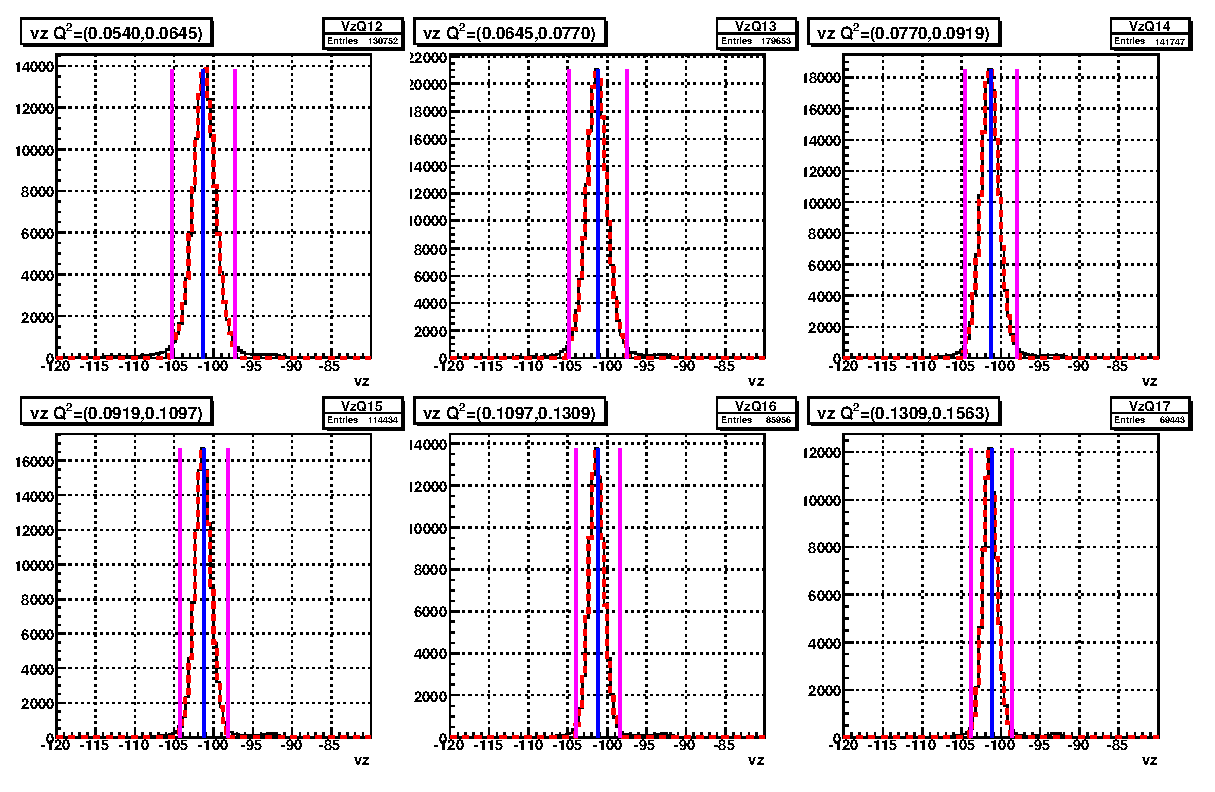
\includegraphics[width=1.0\textwidth]{TexmakerMyFinTh/chap4simul/FigCuts/vzCutsFinalEb2.eps}  %0.6 is the fraction of the real image width????
\leavevmode \includegraphics[width=1.0\textwidth]{TexmakerMyFinTh/chap4simul/FigCuts/vzCutsFinalEb2Ncropped}  %0.6 is the fraction of the real image width????
\caption[v$_z$ cuts (Exp.)]{2.0 GeV data showing the \qsqs dependent v$_z$-cuts (the magenta lines on the left and right of the peaks) in some of the \qsqs bins. The continuous black line represents events before applying all the other event selection cuts (except on v$_z$) and the thicker dotted red line are the events after the cuts. The blue lines are the centers of the distributions, from which the cuts are 3 times $\sigma$ away on each side, where $\sigma$ is the standard deviation for the distribution in the given \qsqs bin (both the central value and the $\sigma$ are determined during the cut development studies).}
\label{vzCtExp}
\end{figure}

As in the case of EC variables, the reconstructed ``v$_z$'' distribution in the simulation does not come out quite the same as in the experimental data %(see the separate section discussing the various issues encountered in simulation). Despite our tremendous efforts, intended agreement in the distributions could not be achieved and to 
. To have the same fraction of events in the corresponding \qsqs bins as in the experimental data, a separate set of cuts (determined based on the distributions of both types of data) had to be used for simulation. For this purpose, the Gaussian fit parameters $\mu$ and $\sigma$ (representing the mean and standard deviation) for all the \qsqs bins were tabulated separately for both data and simulation and separate sets of $\pm 3\sigma$ cuts were determined for all bins. For example, if $\mu_q$ and $\sigma_q$ were the two Gaussian fit parameters for the $q^{th}$ \qsqs bin of either data or simulation, then the lower and upper cuts for ``v$_z$'' for that data set in the given \qsqs bin would be $\mu_q - 3\sigma_q$ and $\mu_q + 3\sigma_q$ respectively (as shown by the magenta vertical lines in Figs. \ref{vzCtExp} and \ref{vzCtSim}.

%\textcolor{red}{My Original Question here was: Should I list all other cuts in a table (may go to Appendix)??}\\
%\textcolor{blue}{You wrote: ``Not sure what you mean''}\\
%\textcolor{red}{Because I showed these \qsq-dependent cuts for only 6 \qsqs bins (in figures), I was wondering if I should list the cuts for other bins in a table somewhere. I guess, may be not.}



\begin{figure}[H]%[h] %ht, htpb (p - float, b = bottom, h=? t = top)
%\leavevmode 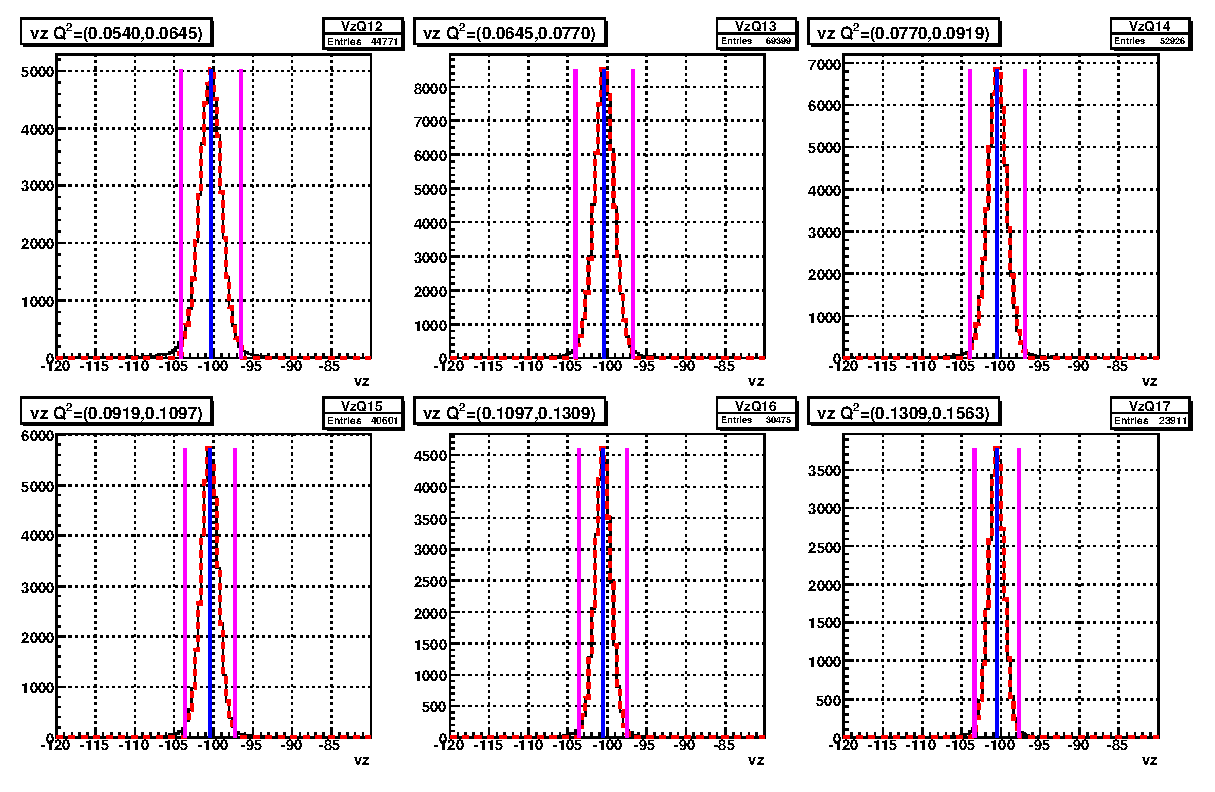
\includegraphics[width=1.0\textwidth]{TexmakerMyFinTh/chap4simul/FigCuts/vzCutsFinalEb2sim.eps}  %0.6 is the fraction of the real image width????
\leavevmode \includegraphics[width=1.0\textwidth]{TexmakerMyFinTh/chap4simul/FigCuts/vzCutsFinalEb2simNcropped}  %0.6 is the fraction of the real image width????
\caption[v$_z$ cuts (Sim.)]{\qsqs dependent v$_z$-cuts on simulation data (similar to Fig. \ref{vzCtExp}).}
\label{vzCtSim}
\end{figure}



%\section{Radiative Corrections}
%Plgiarism Warning: (paraphrasing not done.)
%GSIM - the CLAS Monte Carlo simulation program using GEANT 3.21 libraries from CERN -implements a complete. \cite{clasBrooks}%pg 31 
